\begin{tabular}%
       {|p{3cm}%
        |p{9.5cm}|}
\hline
{\bf Organization Model} &
   {\bf Variant Aspects Worksheet OM-2} \\
\hline
\hline
\sc Structure &
   {\rm
   See Figure~\ref{fig:orgStructure}
   } \\ %TODO
\hline
\sc Process &
   {\rm
   See Figure~\ref{fig:orgProcess}
   } \\ %TODO
\hline
\sc People &
   {\rm
   Single-customer Travel Agent
   } \\
\hline
\sc Resources &
   {\rm \textbf{Database} of locations containing all the available infomation.} \\
 & {\rm \textbf{Database} of customers containing personal features and preferences.} \\
 & {\rm \textbf{Designing software} capable of assembling the itinerary.} \\
\hline
\sc Knowledge &
   {\rm \textbf{Requirement rules}: knowledge to choose a set of locations based on the client features;} \\
 & {\rm \textbf{Preference rules}: knowledge to favour a some location more than others based on client expressed preferences;}\\
 & {\rm \textbf{Constraint rules}: knowledge to exclude or include specific locations based on client explicit directives.}\\
\hline
\sc Culture \& power &
   {\rm The opinion of the client is highly prioritized. Being a small agency no particular power influence is noticeable between co-workers: the hierarchical structure is vertical, with the president occupying the highest position and in charge of all important decisions.} \\
\hline
\end{tabular}

\begin{figure}[h]
\centering
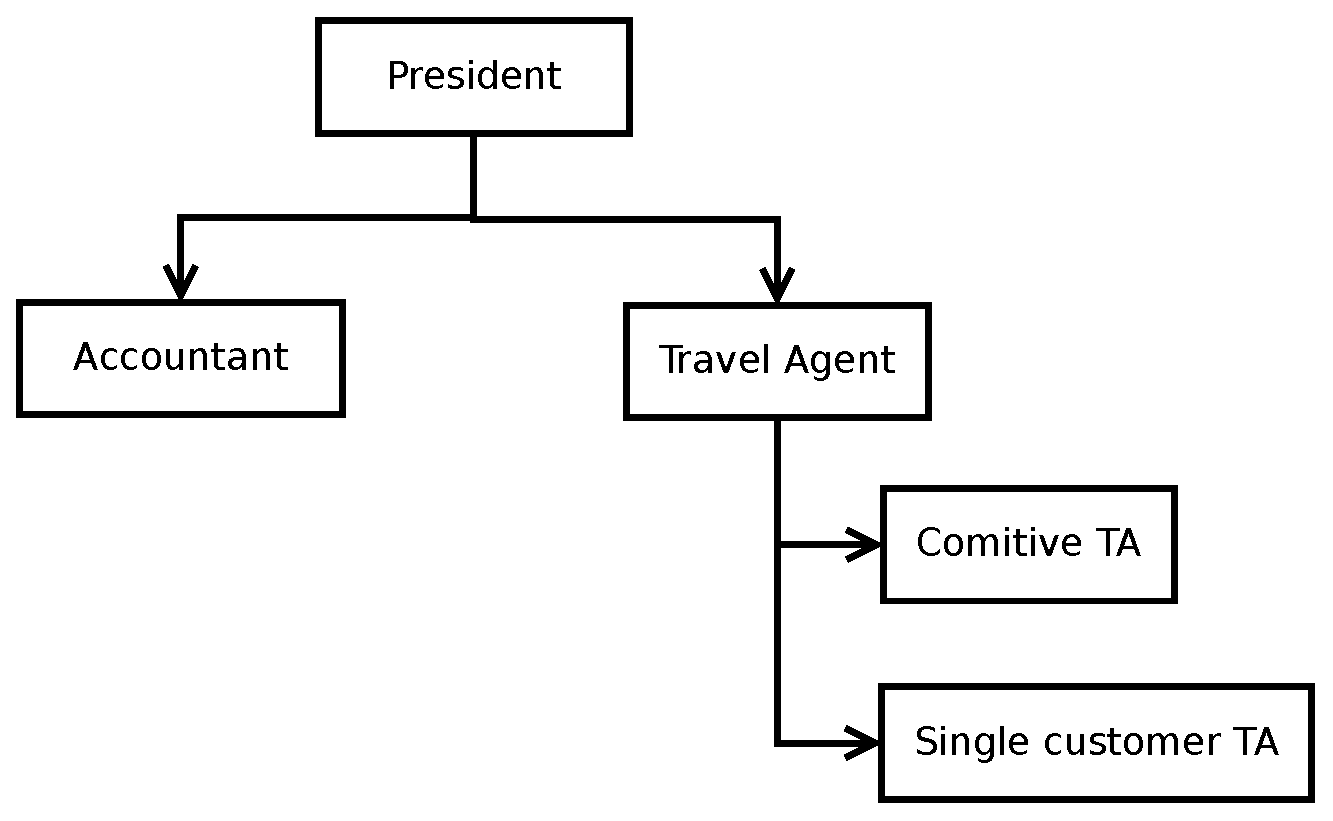
\includegraphics[width=10cm]{images/azienda.eps}
\caption{Organization structure}
\label{fig:orgStructure}
\end{figure}

\begin{figure}[h]
\centering
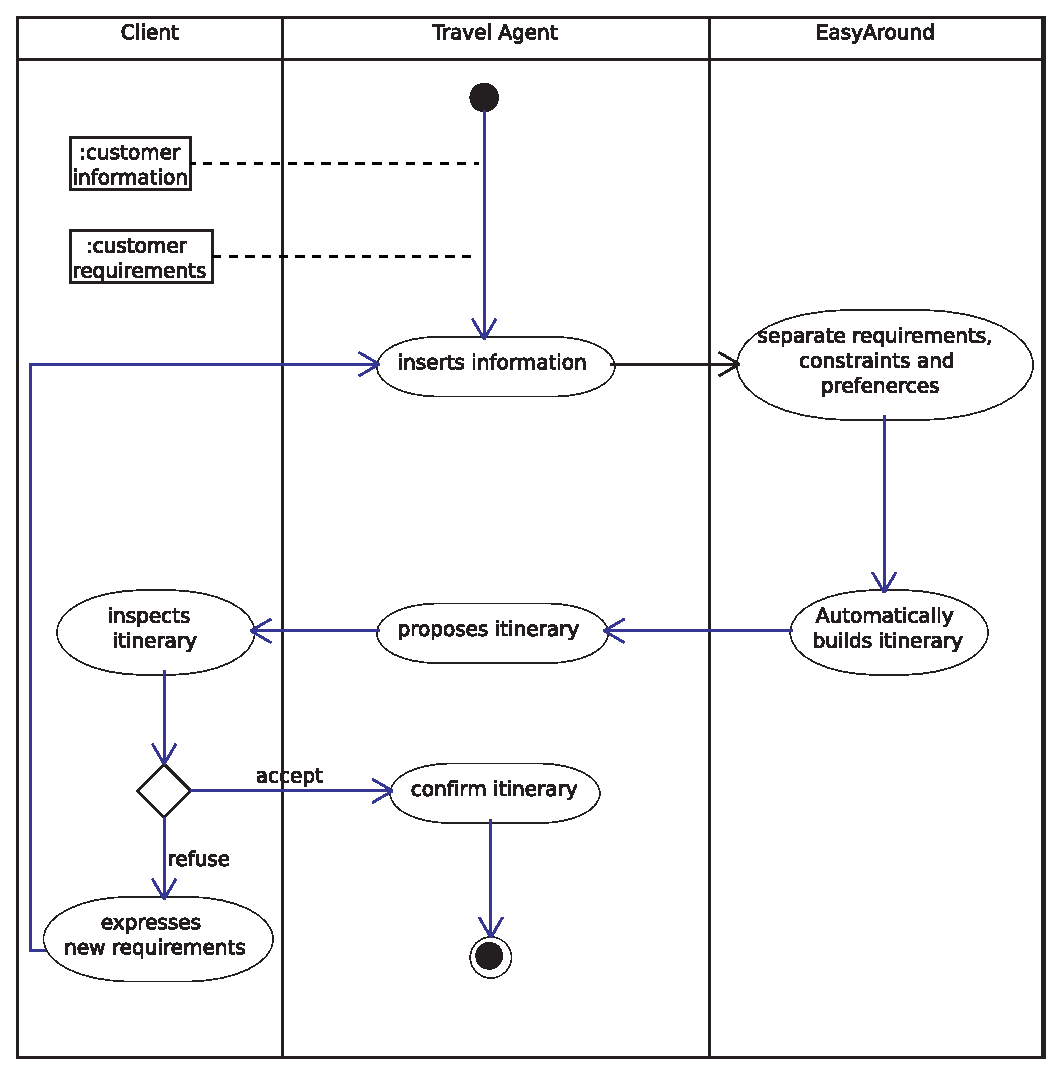
\includegraphics[width=\textwidth]{images/activity.eps}
\caption{Organization process}
\label{fig:orgProcess}
\end{figure}